\chapter{Ensayos y resultados} % Main chapter title

\label{Chapter4}

Este capítulo presenta los ensayos realizados para validar la funcionalidad de
los componentes del sistema, tanto de manera individual como en conjunto. Se
presentan los resultados obtenidos y su análisis.

\section{Banco de pruebas}

El banco de pruebas fue diseñado para verificar el rendimiento, la
funcionalidad y la correcta comunicación entre los sensores, actuadores y
módulos del sistema, en un entorno controlado que simula las condiciones reales
de operación. Incluye los siguientes componentes:

\begin{itemize}
    \item \textbf{Sensores y actuadores:}
          \begin{itemize}
              \item Nodo ambiental: incluye los sensores BMP280, BH1750 y MH-Z19C.
              \item Nodo de consumos: compuesto por un módulo PZEM-004T y seis sensores HC-SR04.
              \item Nodo de solución nutritiva: equipado con un sensor de temperatura DS18B20,
                    sensores de pH, CE, TDS y un sensor HC-SR04.
              \item Nodo actuador: integrado por un módulo de relés de 4 canales (5 V, 10 A) y tres
                    módulos de relés de 2 canales (5 V, 10 A).
          \end{itemize}

    \item \textbf{Microcontroladores:}
          \begin{itemize}
              \item Cuatro módulos ESP-WROOM-32, uno por cada nodo.
              \item Cuatro placas base \cite{PlacaBaseESP32} para los módulos ESP-WROOM-32 para
                    facilitar la conexión de los módulos a los sensores y actuadores.
          \end{itemize}

    \item \textbf{Fuentes de alimentación:}
          \begin{itemize}
              \item Una fuente de 5 V, 2 A para los relés.
              \item Cuatro fuentes de 5 V, 1.5 A para los microcontroladores.
          \end{itemize}

    \item \textbf{Servidor MQTT:}
          \begin{itemize}
              \item El servicio se implementó en AWS IoT Core.
          \end{itemize}

    \item \textbf{Servidor web:}
          \begin{itemize}
              \item El backend, el frontend y la base de datos se desplegaron en una máquina
                    virtual EC2 de AWS, a través del entorno de laboratorio provisto por
                    \textit{AWS Academy Learner Lab}.
          \end{itemize}
\end{itemize}

la tabla \ref{tab:criterios_evaluacion} resume los criterios de evaluación
considerados para la validación del sistema en el banco de pruebas.

\begin{table}[H]
    \centering
    \caption[Criterios de evaluación del banco de pruebas]{Criterios de evaluación del banco de pruebas.}
    \begin{tabular}{p{3.4cm}p{3cm}p{6cm}}
        \hline
        \textbf{Criterio}                          & \textbf{Componente} & \textbf{Descripción}                                                                                                         \\
        \hline
        Verificación de endpoints y almacenamiento & Backend             & Comprobación del funcionamiento de los endpoints y del registro de información en la base de datos.                          \\
        \hline
        Usabilidad de la interfaz web              & Frontend            & Evaluación de la facilidad de uso y el acceso a funcionalidades.                                                             \\
        \hline
        Verificación de mediciones                 & Microcontroladores  & Verificación de los valores reportados por los sensores.                                                                     \\
        \hline
        Activación de actuadores                   & Microcontroladores  & Validación de la activación de los módulos de relés ante eventos enviados.                                                   \\
        \hline
        Verificación de comunicación MQTT          & Comunicación MQTT   & Verificación de la comunicación entre microcontroladores y servidor web a través del intercambio de mensajes en los tópicos. \\
        \hline
        Integración de módulos                     & Todo el sistema     & Verificación del funcionamiento conjunto de sensores, actuadores y servidor web.                                             \\
        \hline
    \end{tabular}
    \label{tab:criterios_evaluacion}
\end{table}

La figura \ref{fig:banco_pruebas} muestra el banco de pruebas utilizado para la
validación del sistema, donde se observan los sensores, actuadores,
microcontroladores y la alimentación eléctrica.

\begin{figure}[H]
    \centering
    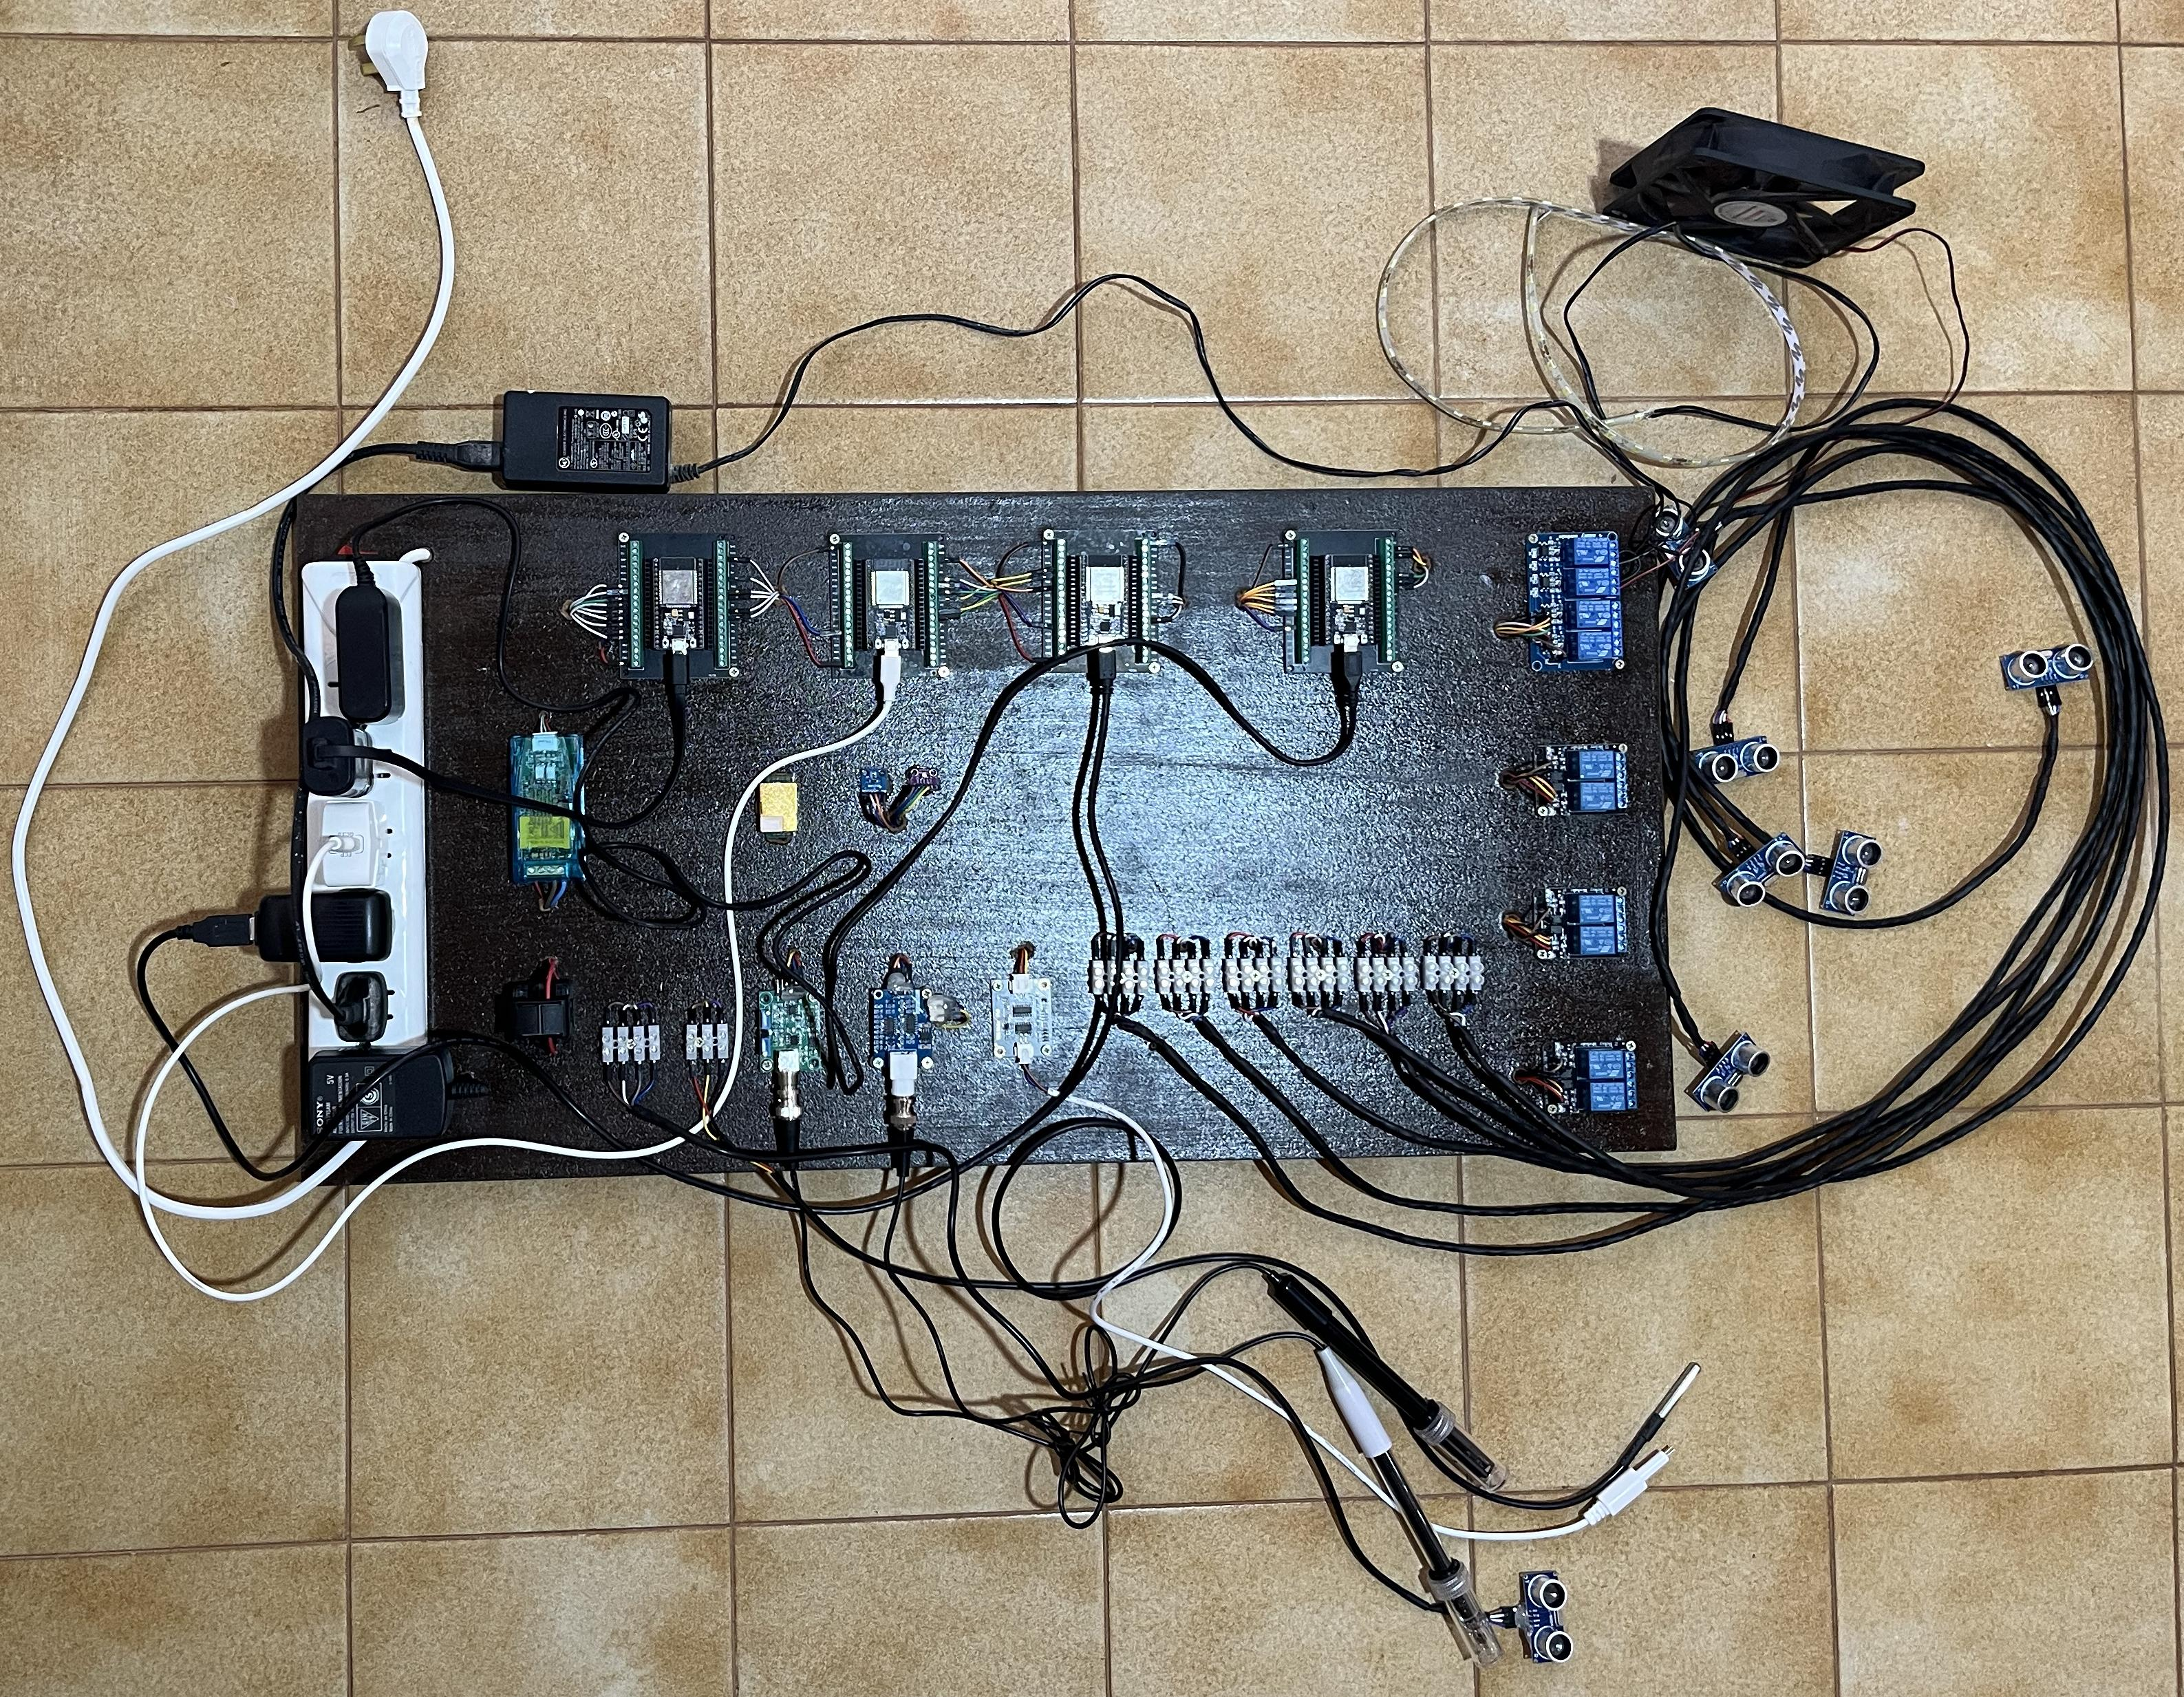
\includegraphics[width=0.95\textwidth]{Images/36_prototipo.jpeg}
    \caption[Banco de pruebas del sistema EnviroSenseIoT]{Banco de pruebas del sistema \texttt{EnviroSenseIoT}.}
    \label{fig:banco_pruebas}
\end{figure}

\section{Pruebas de backend}
\label{sec:pruebas_backend}

Para la validación de todos los endpoints, se empleó la herramienta Postman,
que permitió ejecutar pruebas funcionales. A través de las cuales, se comprobó
que cada endpoint respondiera correctamente a las solicitudes realizadas y
devolviera los datos esperados según la lógica del sistema.

Complementariamente, el backend expone una interfaz Swagger \cite{SwaggerIO},
que facilita la documentación y la validación interactiva de los endpoints.
Esta herramienta permite explorar cada operación disponible, visualizar los
parámetros requeridos y ejecutar pruebas directamente desde el navegador, sin
necesidad de herramientas externas.

La Figura \ref{fig:swagger} muestra la interfaz de Swagger, en la cual se
observan los distintos endpoints disponibles. Cada uno puede expandirse para
acceder a los detalles de la solicitud y la respuesta, así como visualizar
ejemplos y probar su funcionamiento en tiempo real.

\begin{figure}[H]
    \centering
    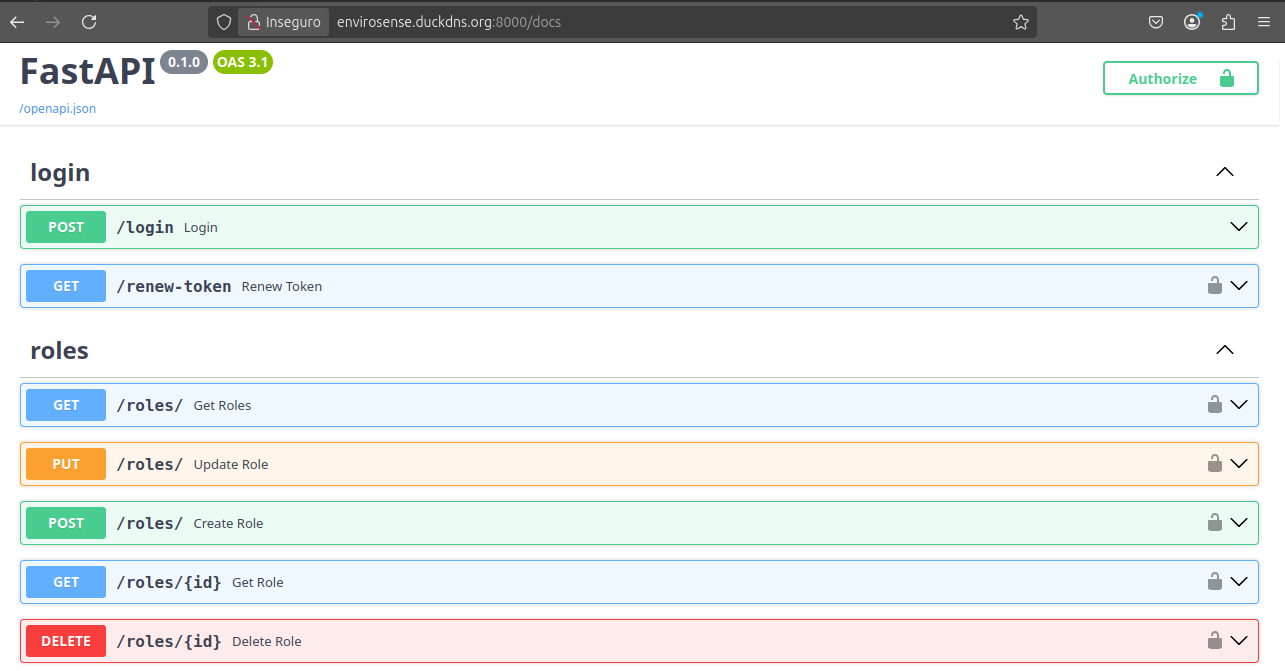
\includegraphics[width=\textwidth]{Images/37_swagger.png}
    \caption[Interfaz de Swagger]{Interfaz de Swagger.}
    \label{fig:swagger}
\end{figure}

\subsection{Pruebas en Postman}

En el repositorio de GitHub \cite{EnviroSenseIoT} se encuentra la carpeta
\texttt{Tests}, que contiene un archivo JSON con la colección completa de
pruebas realizadas con Postman. Dicha colección abarca todos los endpoints del
backend evaluados, junto con los resultados correspondientes.

Tambien se incluye un archivo de texto que resume las pruebas efectuadas, en el
que se detalla los endpoints, los métodos HTTP y los resultados obtenidos, para
permitir una trazabilidad clara del proceso de validación.

La figura \ref{fig:postman} presenta un ejemplo de las pruebas realizadas en
Postman, donde se detalla la respuesta de los endpoints, el método HTTP
utilizado, la URL del endpoint, el código de estado, el tiempo y el tamaño de
la respuesta.

\begin{figure}[H]
    \centering
    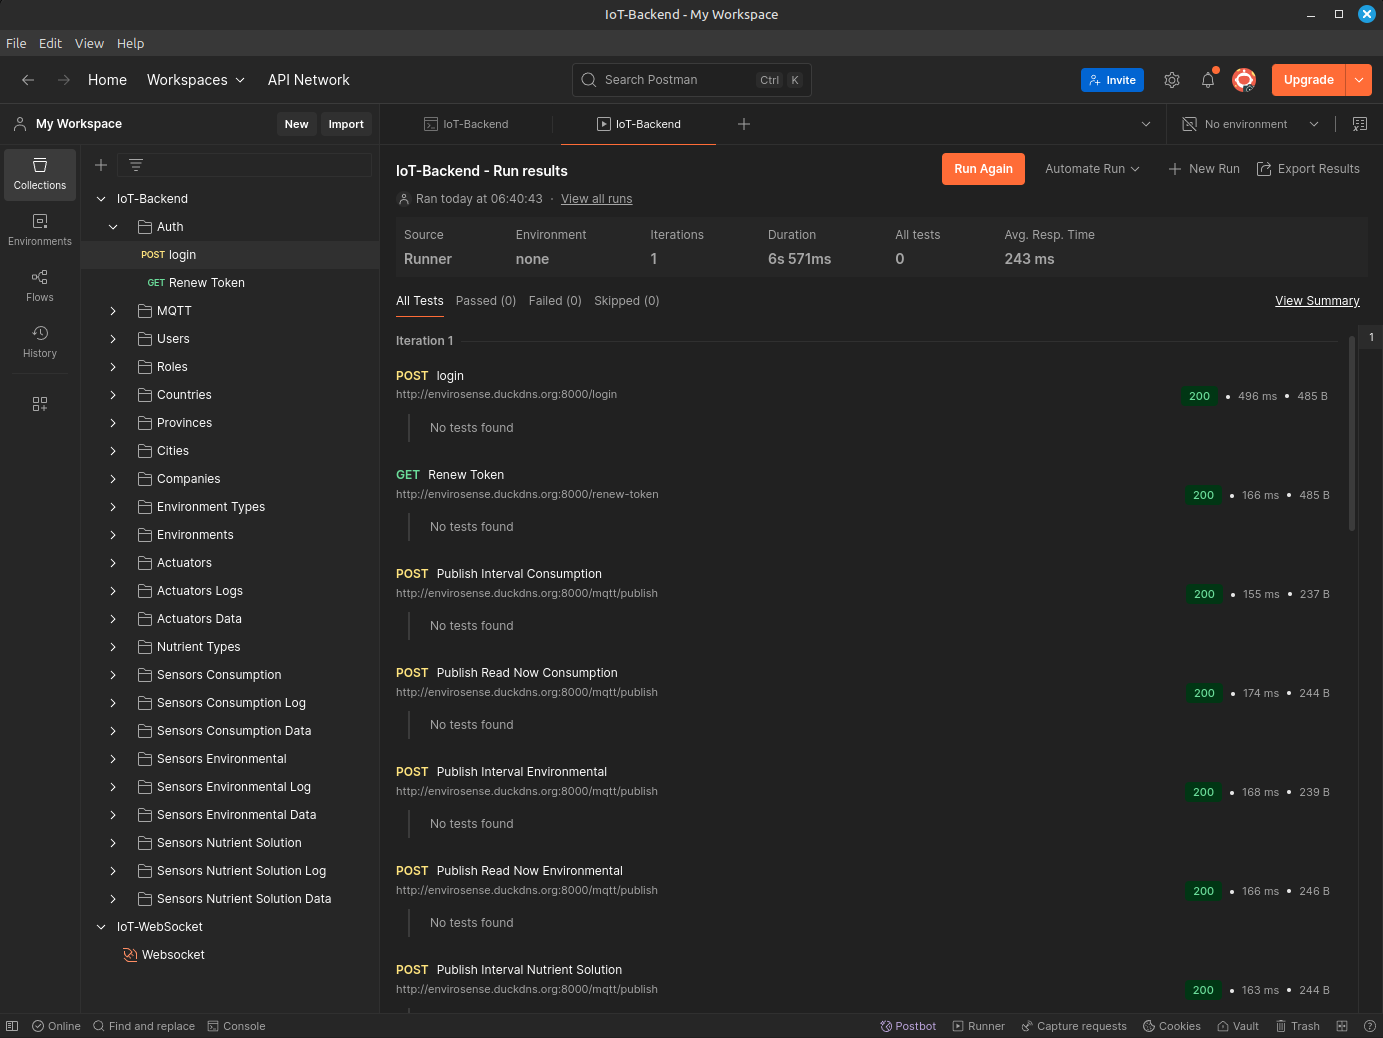
\includegraphics[width=\textwidth]{Images/38_postman.png}
    \caption[Pruebas realizadas en Postman]{Pruebas realizadas en Postman.}
    \label{fig:postman}
\end{figure}

\subsubsection{Evaluación general}

Los tiempos de respuesta obtenidos durante las pruebas fueron, en su mayoría,
adecuados para un entorno con servicios desplegados en contenedores dentro de
una instancia de nube. La latencia promedio se mantuvo entre los 150 ms y 500
ms, valores apropiados para este tipo de arquitectura.

Las operaciones más exigentes, como las consultas con filtros o el cambio de
contraseñas, presentaron tiempos de respuesta ligeramente superiores, aunque
dentro de márgenes razonables considerando la complejidad de dichas acciones y
el entorno de ejecución basado en contenedores Docker.

A continuación, la tabla \ref{tab:tiempos_respuesta} presenta los resultados de
las pruebas realizadas, en las que se evaluaron la funcionalidad y los tiempos
de respuesta de los distintos endpoints. Estas fueron agrupadas en categorías
según la funcionalidad evaluada.

\begin{table}[H]
    \centering
    \caption[Resultados de tiempos de respuesta]{Resultados de tiempos de respuesta de las pruebas.}
    \begin{tabular}{p{5cm}p{5.1cm}p{2.4cm}}
        \toprule
        \textbf{Categoría}                                                     & \textbf{Método}                             & \textbf{Tiempo de Respuesta} \\
        \midrule
        \multirow{3}{5cm}{Autenticación y usuarios}                            & POST Login                                  & 496 ms                       \\
                                                                               & GET Current User                            & 181 ms                       \\
                                                                               & PATCH Update Password                       & 827 ms                       \\
        \hline
        \multirow{3}{5cm}{Publicación de mensajes en MQTT y logs}              & POST Publish MQTT                           & 153 – 181 ms                 \\
                                                                               & GET Logs (actuadores y sensores)            & 173 – 193 ms                 \\
        \hline
        \multirow{2}{5cm}{Consulta de datos de dispositivos}                   & GET Sensors Data                            & $\sim$208 ms                 \\
                                                                               & GET Actuators Data                          & 271 ms                       \\
        \hline
        \multirow{3}{5cm}{Operaciones de creación, modificación y eliminación} & POST Create User / Company                  & $\sim$490 ms                 \\
                                                                               & POST Create Sensor / Data                   & 154 – 194 ms                 \\
                                                                               & PUT / DELETE                                & 161 – 188 ms                 \\
        \hline
        \multirow{4}{5cm}{Datos geográficos y configuración}                   & GET Countries / Provinces / Cities          & 176 – 187 ms                 \\
                                                                               & POST Create Environment / Actuator / Sensor & 179 – 194 ms                 \\
        \bottomrule
    \end{tabular}
    \label{tab:tiempos_respuesta}
\end{table}

\subsubsection{Resultados generales de las pruebas}

El siguiente listado resume los resultados de las pruebas realizadas en
Postman:

\begin{itemize}
    \item Todas las pruebas fueron completadas de manera exitosa, sin errores de backend
          ni fallos de respuesta.
    \item Los tiempos de respuesta fueron consistentes y apropiados para un sistema
          desplegado en contenedores sobre infraestructura en la nube.
    \item Las operaciones críticas (autenticación, creación de entidades, consultas de
          datos) respondieron dentro de márgenes adecuados para el entorno de prueba con
          el servicio en la nube.
\end{itemize}

\subsection{Pruebas de validación de almacenamiento en MongoDB}

Se llevaron a cabo pruebas para validar el almacenamiento de datos en MongoDB,
con el objetivo de comprobar que las operaciones de escritura realizadas desde
el backend, tales como la creación de usuarios, sensores, mediciones y eventos,
se registraran en las colecciones correspondientes.

Para ello, se realizaron las siguientes acciones:

\begin{itemize}
    \item Se ejecutaron operaciones desde Postman, para generar nuevas entidades en el
          sistema.
    \item A continuación, se accedió directamente a la base de datos MongoDB, a través de
          la herramienta MongoDB Compass \cite{MongoDBCompass}, para inspeccionar las
          colecciones y verificar la existencia y la estructura de los documentos
          insertados.
    \item Se validó que las operaciones de actualización y eliminación impactaran
          correctamente sobre los documentos correspondientes en MongoDB.
\end{itemize}

Estas validaciones permitieron confirmar que el backend realiza una correcta
persistencia de los datos en MongoDB y que no se observaron inconsistencias, ni
pérdidas de información durante las operaciones.

La figura \ref{fig:mongodb} ilustra un ejemplo del proceso de creación de un
nuevo usuario. Se muestra la solicitud enviada desde Postman junto con la
respuesta proporcionada por el servidor. Asimismo, en la interfaz de MongoDB
Compass se visualiza el nuevo usuario incorporado en la colección \texttt{User}
de la base de datos.

\begin{figure}[H]
    \centering
    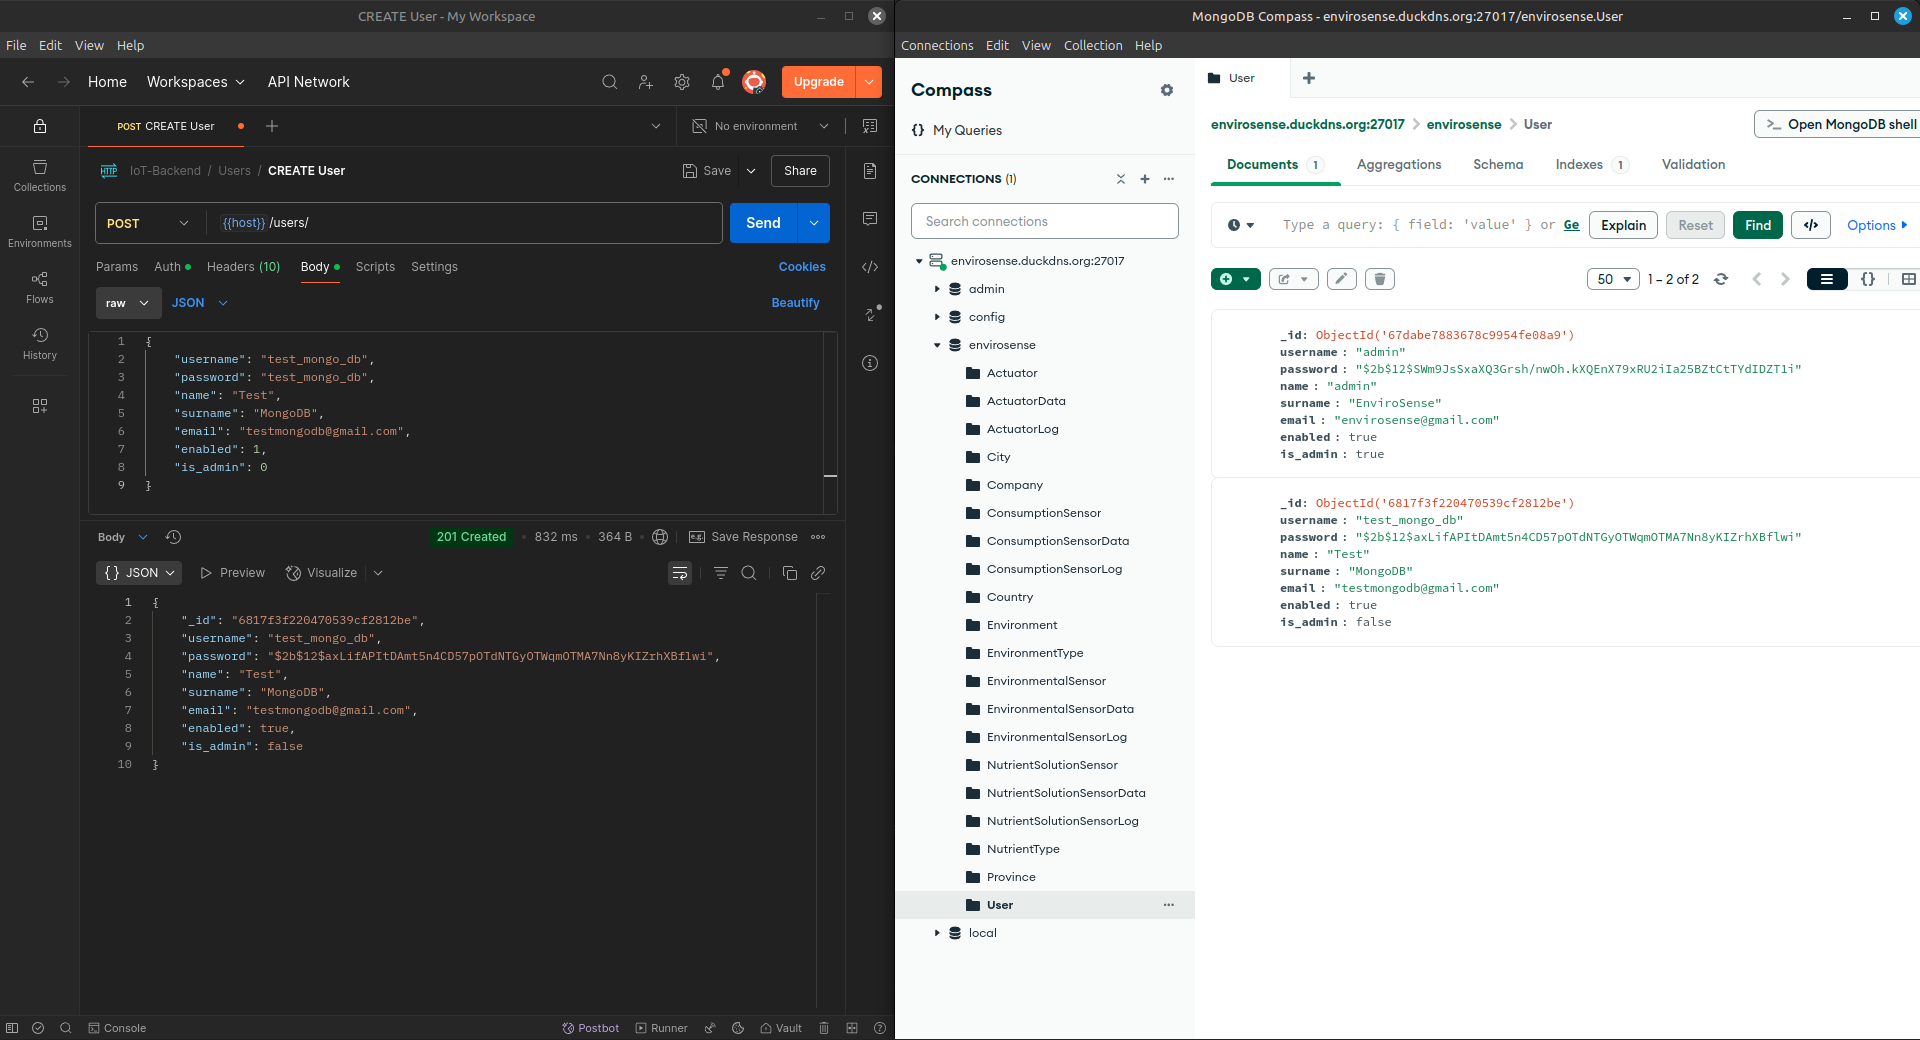
\includegraphics[width=\textwidth]{Images/39_test_mongodb.png}
    \caption[Validación de almacenamiento en MongoDB]{Validación de almacenamiento en MongoDB.}
    \label{fig:mongodb}
\end{figure}

\subsection{Resumen de pruebas del backend}

Las pruebas efectuadas sobre el backend confirmaron el correcto funcionamiento
y la capacidad para responder adecuadamente a las distintas solicitudes. Los
tiempos de respuesta se mantuvieron dentro de los rangos esperados y se
verificó con éxito la persistencia de los datos en MongoDB.

